%%%%%%%%%%%%%%%%%%%%%%%%%%%%%%%%%%%%%%%%%
% Stylish Article
% LaTeX Template
% Version 2.1 (1/10/15)
%
% This template has been downloaded from:
% http://www.LaTeXTemplates.com
%
% Original author:
% Mathias Legrand (legrand.mathias@gmail.com) 
% With extensive modifications by:
% Vel (vel@latextemplates.com)
% Final ACS by:
% Juan Barbosa
% License:
% CC BY-NC-SA 3.0 (http://creativecommons.org/licenses/by-nc-sa/3.0/)
%
%%%%%%%%%%%%%%%%%%%%%%%%%%%%%%%%%%%%%%%%%
\documentclass[fleqn,11pt]{SelfArx}
%\usepackage[superscript]{cite}
\usepackage{wrapfig}
\usepackage{rotating}
\usepackage{subcaption}
\usepackage[numbers, super]{natbib}
%----------------------------------------------------------------------------------------
%	ARTICLE INFORMATION
%----------------------------------------------------------------------------------------

\JournalInfo{Laboratorio Org\'anica 3, No. 4, 14/10/2017} % Journal information
\Archive{ }

\PaperTitle{Acilación de Friedel-Craft} %
%\Keywords{Keyword1 --- Keyword2 --- Keyword3} % Keywords - if you don't want any simply remove all the text between the curly brackets
%\newcommand{\keywordname}{Keywords} % Defines the keywords heading name

%----------------------------------------------------------------------------------------
%	ABSTRACT
%----------------------------------------------------------------------------------------

\Abstract{
\begin{wrapfigure}{r}{0.45\textwidth}
	\centering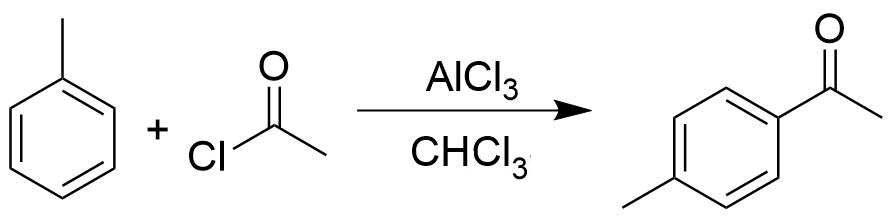
\includegraphics[width=0.95\linewidth]{structures/reaction.png}
\end{wrapfigure}
}

%----------------------------------------------------------------------------------------

\begin{document}

\flushbottom % Makes all text pages the same height

\maketitle % Print the title and abstract box

%\tableofcontents % Print the contents section

\thispagestyle{empty} % Removes page numbering from the first page
\renewcommand{\tablename}{Tabla} 


%----------------------------------------------------------------------------------------
%	ARTICLE CONTENTS
%----------------------------------------------------------------------------------------

\section*{Introducci\'on} % The \section*{} command stops section numbering
%------------------------------------------------


\section{Resultados y Discusi\'on}
\section{Conclusiones}

\section{Secci\'on experimental}

%----------------------------------------------------------------------------------------
%	REFERENCE LIST
%----------------------------------------------------------------------------------------
%\newpage
\phantomsection
\bibliography{informe}
\bibliographystyle{achemso}

%----------------------------------------------------------------------------------------
\onecolumn
\section{Informaci\'on suplementaria}\label{sec: complementaria}
\end{document}